\documentclass[a4paper,10pt,twoside]{report}
\usepackage{color}
\usepackage[utf8x]{inputenc}
\usepackage[english]{babel}
\usepackage[T1]{fontenc}


%% font
\usepackage{palatino}

% url
\usepackage{url} 

% fancy
\usepackage{fancyhdr}

% for listing codes
\usepackage{listings}

% for import pictures
\usepackage{graphicx}

\usepackage[colorlinks=true,linkcolor=blue,citecolor=blue,urlcolor=blue]{hyperref}
\usepackage{anysize}


\marginsize{22mm}{14mm}{12mm}{25mm}

%% for import a bibliography
\usepackage{natbib}

%%%%%%%%%%%%%%%%%%%%%%%%%%%%%%%%%%%%%%
%% to quote a figure:
\newcommand{\figref}[1]{figure~\ref{#1}}

%% to quote citation
\newcommand{\Ref}[1]{(\ref{#1})}

%% to emphasize a word or phrase:
\newcommand{\empha}[1]{\textit{\textbf{#1}}}

%% differential operators:
\newcommand{\D}{\partial}
\newcommand{\Dt}{\partial_t}
\newcommand{\Dx}{\partial_x}
\newcommand{\Dy}{\partial_y}


%%%% start macro to remove the chapter name %%%%
\makeatletter
\def\@makechapterhead#1{%
  \vspace*{0\p@}%
  {\parindent \z@ \raggedright \normalfont
    \interlinepenalty\@M
    \ifnum \c@secnumdepth >\m@ne
        \Huge\bfseries \thechapter\quad
    \fi
    \Huge \bfseries #1\par\nobreak
    \vskip 40\p@
  }}

\def\@makeschapterhead#1{%
  \vspace*{0\p@}%
  {\parindent \z@ \raggedright
    \normalfont
    \interlinepenalty\@M
    \Huge \bfseries  #1\par\nobreak
    \vskip 40\p@
  }}
\makeatother
%%%% end macro %%%%


\renewcommand{\baselinestretch}{1.30}\small \normalsize
\renewcommand{\baselinestretch}{1.18}\small \normalsize

\renewcommand{\chaptermark}[1]{%
	\markboth{#1}{}}


\fancyhead[LO,RE]{\leftmark}

\fancyhead[LE,RO]{\rightmark}

\fancyhead[LE,RO]{}
\fancyfoot[CE]{\thepage}


\setcounter{tocdepth}{1}     % In the table of contents


\renewcommand{\thechapter}{\Roman{chapter}}
\renewcommand{\thesubsection}{\Alph{subsection}}

\renewcommand{\sectionmark}[1]{\markboth{#1}{}}
\renewcommand{\subsectionmark}[1]{\markright{#1}}

\title
{
	\vspace{20mm}
	\large{Master 1 ALMA\\
	Techniques de Développement\\
	2009-2010}\\
	\vspace{15mm}
	\Huge{Technical Documentation}
}
\author{Frédéric Dumonceaux\\Frédéric Dumont}
	\vspace{45mm}

\begin{document}

\addcontentsline{toc}{chapter}{Abstract}

\thispagestyle{empty}

\maketitle

\tableofcontents

\newpage

\pagestyle{fancy}

\chapter*{Preface\markboth{Abstract}{}}


	The game of Go is native to China. It confronts two opponents who place alternately black and white stones on a goban called goban. Players trying to gain control of the game plan and build territories. Each player is trying to encircle the stones of his opponents and capture them to enlarge its territories.\\

	Putting stones close enough to each other, allow them to support themselves and avoid capture. On the other hand, placing stones far away as possible from each other creates an influence on the goban. Much of the difficulty of this game comes from the need to find a balance between several conflicting interests. Each player must try to be both offensive and defensive and to choose between the urgent short-term tactical and strategic choices of long-term.\\

	Its success owes as much to the simplicity of its rules at its rich combinatorial and strategic depth.\\

	We propose here to present our implementation of a variant of the game of go based not on the number of territories conquered but the number of stones captured during a game, better known under the name of the atari-go.

\section*{Readership}
\addcontentsline{toc}{section}{Readership}
\vspace{4mm}

	This document is aimed at two categories of users of our program, according to the following needs:\\
	
	\begin{itemize}
	\vspace{4mm}
		\item{Developers $\Rightarrow$  Here they will find enough information to potentially alter the interface and the various modules making up the IA or the internal data structures. Some references to publications on the theme of the game of go are also given in the bibliography. They will explain some choices in the logic used. The terms specific to the game of go are presented in the first chapter.}\\

		\item{Users $\Rightarrow$  We consider here, all and sundry who wish to play either against the computer or against a human player. The installation and execution of the program by a virtual machine will be presented.}
	\end{itemize}
	\vspace{4mm}

    We will ignore the intricacies of the system, therefore methods of implementation and other internal algorithms, which will interest the developers wishing to improve the application. They will find in the \emph{ad hoc} chapters, formal specifications of structures used for its implementation and motivation around the choices of implementations.

\section*{Guide Organization}
\addcontentsline{toc}{section}{Guide Organization}
\vspace{4mm}

	    Consistent with the foregoing, we shall have the chapters with their content in the following list:\\

    \paragraph{Chapter 1, \emph{Basics}}
	~~\vspace{2mm}
	
	This chapter presents the specific terms of go and those generally used in the literature about programming the game of go. A quick reminder on the rules of the game will be also done.

	\paragraph{Chapter 2, \emph{Structures of the application}}
	~~\vspace{2mm}
	
	We briefly present the different data structures and links between them. On donnera également la façon pour étendre facilement l'infrastructure et l'augmenter.We will also give the way to easily extend the infrastructure and increase it.

	\paragraph{Chapter 3, \emph{Evaluation methods}}
	~~\vspace{2mm}
	
	This chapter will be devoted to the methods deployed by the software to recognize certain situations on a goban at a given moment of play.

	\paragraph{Chapter 4, \emph{Software use}}
	~~\vspace{2mm}
	
	Finally, we found the tutorial to start and use our application with its graphical interface.


\chapter{Basics}

	We present in this chapter some basic concepts about the game of go and the development of a reliable model. As recalled in \cite{Bouzy2001}, the problems of life and death are problems that happen when a group of stones is completely encircled. This problem is crucial since it allows to say which groups are alive or dead and where to play.\\

	Other related concepts are highlighted in \cite{Bouzy95} like that of enmity or emptiness. Similarly, each of these concepts appear at certain levels, those previously cited are clearly high-level and model the state of a group of stones. The following sections describe the concepts we have implemented in our application after studying how to model them.

\section{Different games}
\vspace{4mm}


	We consider a game as part of a problem, which we seek to determine a configuration leading to a very specific purpose. The aggregation of several games can move from an elementary level to a  level iterative, gathering stones in groups and forming territories.\\

	At the elementary level, we have the connection set and the separation of the chain. Similarly, we use Conway's notation to specify the possibility that the game configuration lead up to the desired result always by placing themselves to the point of view of the player, playing the next move:
	\vspace{3mm}
	
	\begin{itemize}
		\item[$>$]{ : this connector leads that the game is won, no matter who will play the next move;}
		\vspace{1mm}
		\item[$\star$]{ : this connector leads that the game can be won if the player plays the next shot, which means that the opponent can possibly block the next.}
		\vspace{3mm}
	\end{itemize}

	We'll use these connectors to describe a specific game and deduce its quality. Note also that the connector $<$ has a semantics, but that is not employed in this case.

	\paragraph{Connection}
	~~\vspace{2mm}
	
	The connection is used to define strings and is useful for creating groups of stones, base of the game of go. For a given game, we consider a set of disjointed friends stones, not being in contact directly. We consider the game as we can aggregate multiple stones so that it forms only a single group. This implies that it shares at least one common liberty to have a chance to connect, regardless of the presence of opponent's stones.
	
	\paragraph{Separation}
	~~\vspace{2mm}

	The game of separation is the \emph{dual} of the game of the connection. We are trying here to prevent the opponent to connect his stones to form chains. The game consists to find two chains of stones so that they can not connect to a restricted set of intersections of the goban. Success depends on the number of possibilities and the position of the ends of two chains (which can be reduced for each composed of a single stone).\\

	We easily deduce that play a connection comes down to play a separation. Indeed, once several stones friends can connect, they may also separate adversary so underlying : the topological concept of the connection is the 4-connexities, but the separation rather uses the 8-connexities (two stones in diagonal lines are sufficient to separate two opposing strings). So, a set of stone in chain may be completely encircled by a 8-connected set, hence the importance of this concept and its close relationship with the connection.

	\paragraph{The Eye}
	~~\vspace{2mm}

	The eye is an important figure in the game of go because it can give a quantitative and qualitative measure of health to a chain of stone. The creation of this figure requires that a string around an empty intersection, so that this chain can be taken only by emphasizing the intersection. Indeed, the opposing player must first wrap the string and then play on the eye itself, which is prohibited by default, except if a stone is captured consecutively to the laying of the stone. We deduce a chain with two eyes is so invulnerable because we can play on two eyes during the same phase of play, hence the importance of this figure.\\

	Except for the game of the eye, each of its games can be used on a larger scale, to a level says "iteratif" and allow more complex structures, useful for the concept of encirclement. For this project, we have limited ourselves to the implementation of elementary games and we will present our construction methods.


\chapter{Structures of the application}


	The development of the application was made following two distinct parts. On the one hand, we have the game engine that manages the specific structures (goban, positions, groups,\ldots) and artificial intelligence. Secondly, the Graphical User Interface. We will describe and attempt to justify, for each, our choices of implementation. For more details on the application code, it is advised to refer directly to these sources and the  \emph{javadoc}, adequately commented for better understanding.

	\section{Development of AI} 
	\vspace{4mm}

	The game of Go is considered as a complex problem in artificial intelligence, which can not be solved easily unlike chess. This may seem like to be a problem more complicated than the game of go, because of the complexity of the rules of the game. In reality, the rules of the game of go is due to the combinatorial explosion induced by the large number of playable position and thus the number of structures allowed over a game.\\

The game programs of go fail to reach the current average level of amateur players of go. On small goban 9x9, the best programs have recently reached the level of players dan, but the techniques that have allowed this growth have yielded only mixed results on a goban 19x19. This shows the difficulty of creating an artificial intelligence for this game. However, as part of this project, we have striven to achieve an artificial intelligence capable of playing well against a human player on a goban 9x9.\\

	We therefore divided our application in specific modules:
	\vspace{3mm}

	\begin{itemize}
		\item{Position :this module is shared by the goban and groups of stones, it symbolizes the state of an intersection on the goban and thus the nature of a stone covering this intersection, if this is the case ;}
		\vspace{1mm}
		\item{Coord : This module allows to define the coordinates of windows on the goban and identify groups of stones on a subset and make calculations of intersections ;}
		\vspace{1mm}
		\item{Move : This module represents a move played and contains the reference to the state of the goban that it modifies, coordinates of move and the resulting valuation ;}
		\vspace{1mm}
		\item{Tree et Node : These two modules allow the representation of tree and storage of move played and implementations of the  algorithm min-max and alpha-beta ;}
		\vspace{1mm}
		\item{StoneGroup : This module is the aggregation of a set of 4-connected positions and positions occupied on the goban, it also contains the list of border stones of a group and its liberties ;}
		\vspace{1mm}
		\item{State : This module represents the class of higher-level since it contains the goban itself and has methods ensuring the observance of the rules of the game and evaluation of its current state using appropriate methods ;}
	\end{itemize}

	\paragraph{Position}
	~~\vspace{2mm}

	We consider as position of goban, a busy intersection or not of this goban. Each position has the information to its original state and eventually the group it belongs if it is occupied by a stone. We also demonstrated that an empty intersection could be adjacent to one or more groups of stones. When this is true, we also maintain a list of references to these adjacent groups, allowing us to have an idea of the influence around certain intersections and allowing us to use for example in the detection of eye, that we will detail in Chapter 3.

	
	\paragraph{A group of stones}
	~~\vspace{2mm}


	We consider as a group of stones, all non-empty intersections of Goban, of the same color and 4-connected locally. To this we also add a list of references to the stones that border the group of stones and the list of positions that are empty localy at the group in question. We also maintain the extreme positions of the group, who permit to know if windows of two groups intersect, without guaranteeing that if this is true, there is adjacency of these on one of their liberty. On the other hand, we know immediately if this does not happen, groups can not be adjacent and we will not need to measure the influence of one over the other. We also provide methods for measuring the connectivity of one group over another on 4-connected liberties or 8-connected liberties (useful for separating), we have a method to measure the influence of opposing groups on two groups friends. Finally, we maintain the list of the eyes of the group that remains valid, until the group is alive or that we do not add stones at those positions.

	Each information described here is built for each new move played on the goban and is therefore controlled by a state of the game.

	\paragraph{A State}
	~~\vspace{2mm}

	A state is the module that controls all other. It contains the array of original positions of goban and the list of groups of black and white stones placed on the board. It is responsible for verifying whether a move is legal, according to the rules of the game. Moreover, if a move is made, it monitors the implementation of this move and edge effects induced : first, we check if the earlier position was an eye, thus, the group in which he belonged loses it. Then, if the stone is added to close friends groups (its neighbors are on their own liberties), we add it to the first found then we merge in turn all groups to have a single since forming a new string 4-connected. If necessary, liberties are recalculated, boundaries of each group are modified and we take care to eliminate, those without any more.\\

	This unit also includes the basic methods for the creation of artificial intelligence. To create this intelligence, we have therefore used the algorithms min-max and alpha-beta. We have a specific method, from the first move, the method will create the tree of following states at a depth fixed in advance. For each starting node (corresponding to a state), we seek its best sons (depending on the evaluation function) that is added in a priority queue. Once all the moves played, We start again the algorithm on them to reach the desired depth for the algorithm of depth research, new son is not treated from a certain depth and the queue containing them empties.\\

	Then, a method goes up the value of the minimum and the value of the maximum to the root, using the method of pruning (alpha-beta) if necessary. The method of calculating the next move to play returns the parent node which contains the quantitative assessment and details of the best next move to play.\\

	The next chapter will describe the internal methods for measuring the state of the game

	\section{Class diagram of the engine} 

	The following diagram shows the interactions between different modules of the engine:
	\begin{figure}[htb!]
	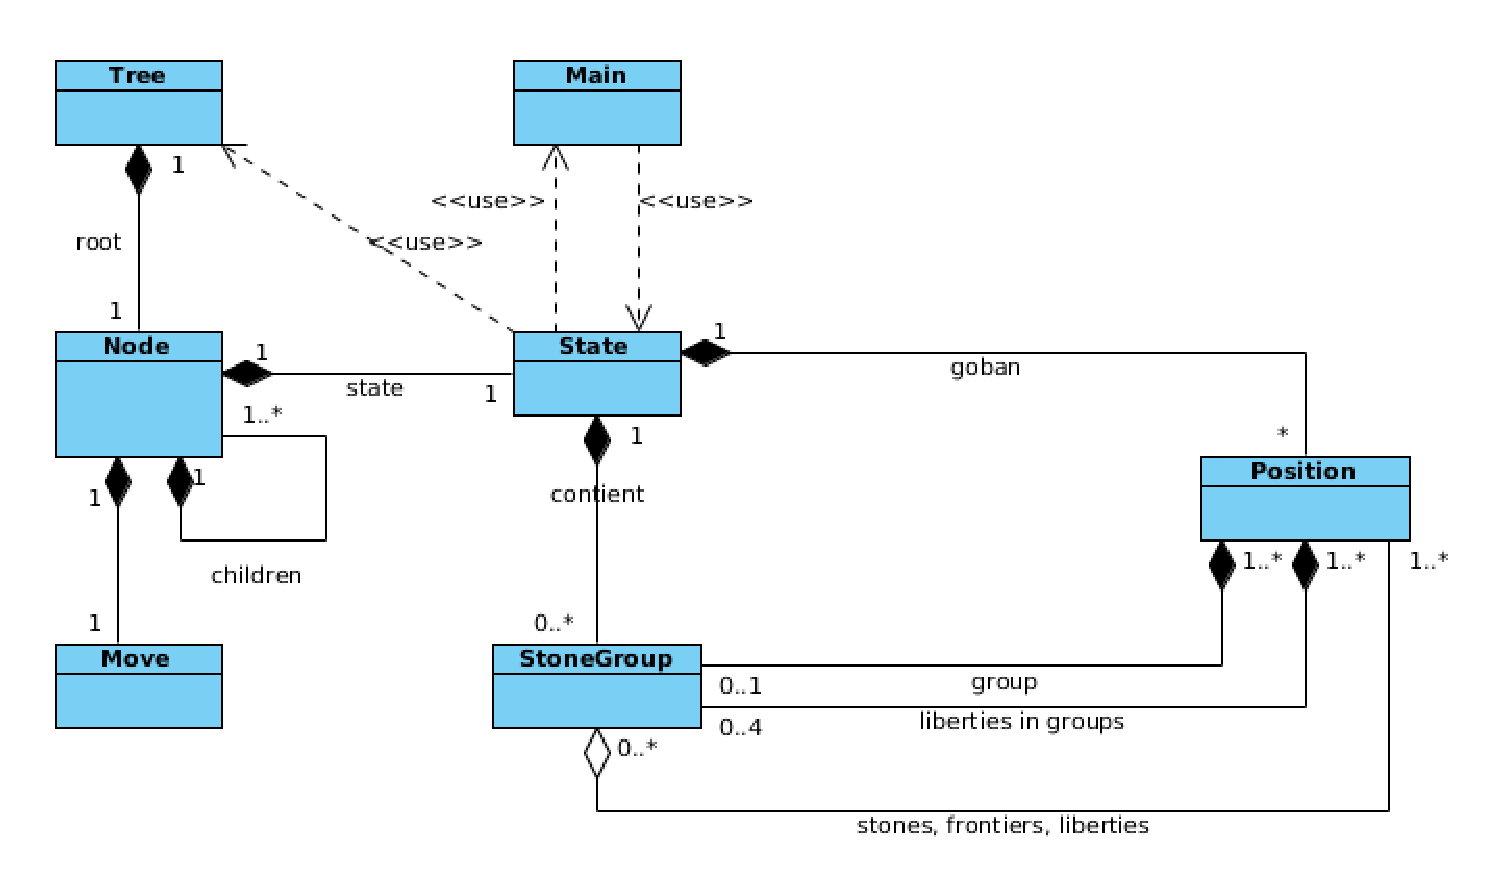
\includegraphics[width=17.5cm]{diagram_class}

	\caption{Class diagram}
	\label{fig:class}
	\end{figure}

As shown, the class \textbf{Main} is instantiated to launch the application, it is linked to the GUI. It contains an attribute for the current state of play and allows the construction of a search tree for the next move to play (case in which the computer is called to play). The tree contains a root node of all other and each node has a set of son. Each node is linked to a specific state and a possible move, itself symbolized by two coordinates of the space of the goban. When applying the algorithm the state of the root node replaces the current state, characterizing the moves played by the computer.\\

	At engine, we found strong links around the trio \textbf{State}, \textbf{StoneGroup} et \textbf{Position}. A set of positions is linked to a state for the entire lifetime of the application and represents each position of the Goban. a parameter permits to say if the position is empty or busy by a stone and what type of stone occupies this position. The addition of stones on the board, involves the creation of groups of stones that contain the positions of goban for liberties, the border and the stones themselves ; the border is always a subset of stones and can be equal as the number of stones does not exceed four, this is true since no stone can not be deprived of its four liberties by its neighbors.\\

	As shown in the diagram,positions exist independently of groups of stones that can disappear of the goban. However, this withdrawal has the effect of resetting the positions to "empty". Moreover, we add a double composition between a position and, a group or a set of groups. The first composition symbolizes the link between a position and its membership in a group of stone, as being itself one, or being a liberty. The second exists only when the position is an empty intersection and represents adjacent groups (on its 4-connected liberties), and as stated above, is a measure of the influence of groups on the goban. Note that these two compositions may exist at the same time when the intersection is empty : indeed, if the intersection has one or more adjacent groups, therefore it is part of the freedoms of each of these groups.  

	\section{GUI Development} 
	\vspace{4mm}

	The interface has been realized in Swing. It is a graphics library for the programming language Java. Swing offers the possibility to create graphical identical user interfaces whatever the operating system underlying. Thus, the program is usable on any platform.\\

	To create the interface for this application, we have defined different classes. In this section, we do not fully detail all classes implemented for the interface, but we will specify the features they include. To know more fully the different implementations, just look at the Javadoc or visit the code directly.

	\paragraph{class Main}
	~~\vspace{2mm}

	This class allows the creation of a graphic window (global container \emph{JFrame}) may contain any other container or graphics element that we want to display. Thus, we have created a menu to manage a variety of options such as the number of players or the difficulty of the game for example. Following this menu, we have associated at this window a independent container  (container \emph{JPanel}) for the representation of the goban. Finally, we have added a status bar to find information about the current game, a progress bar and a button. This last two elements are useful in a game against the computer. Indeed, the progress bar permits to know the state of the search for a move to play and the button can stop this search. Once the button is pressed, the computer will play the best move it has previously found.

	\paragraph{class Goban}
	~~\vspace{2mm}

	This class allows the creation of a container \emph{JPanel} in which we create the Goban. The establishment of the Goban is special. Indeed, when creating a new goban, we also create a new game. The game's role is to create an array of moves that will record the different states of the boxes of the Goban (whether a particular box has a stone, the color of the stone, etc..). Thus the table gives information about the state of the Goban. The method \textbf{paintComponent} is the main method of the \emph{JPanel}. So in this method we do all the processing for displaying the various elements. The method \textbf{rezise} redefines the elements of different sizes if required (enlargement of the window), We also call on other methods to display different lines, display different stones of the goban (by searching in the table explained previously) and display the background image of the goban.\\

	The Goban must interact with the user via the mouse. for this, we have defined other methods to permit this interaction. Thus, when moving the mouse, a transparent stone indicates what move we can play depending on the location of the cursor via the method \textbf{mouseMoved}. At a click, the method associated with this event \textbf{mouseClicked}, calls other methods, for example, retrieve the coordinates of the mouse (to know the position of the stone in the Goban), whether the move is valid, to update the table of movements (add or remove), display the stone on the board if possible and/or remove (if one or more stones are captured).


	\paragraph{classe Game}
	~~\vspace{2mm}

	This class allows the creation of an array of movements. this array includes the state of the boxes of the goban (if a particular box is empty or if a stone is placed). They have different methods which  the main are \textbf{stop} who allows to empty the table of movements (in the case of a new game), and \textbf{newStoneMove} who allows to add a new move in the table of movements. 

	
	\paragraph{classe Button}
	~~\vspace{2mm}

	This class allows the creation of a button. The button offers the possibility to stop the search of a new move played by the computer during a game against it. To achieve this, we defined an action to perform when the button is pressed. This action is performed in the method \textbf{actionPerformed}.


\chapter{Evaluation methods}


	This chapter will attempt to describe the methods used to recognize from a state of the game, power struggle between groups of stones and links with the methods of implementations and backups of information explained in the previous chapter.\\

	The previous chapter introduces our methodology to implement the methods which the evaluation focuses on a particular concept of a current state , explaining his delegation to the class \textbf{State}.

	However, at this stage, if these functions prove correct and functional for any state of the Goban, we have not had time to establish quantitative measures associated ; Indeed, they convey just one qualitative information according to the point of view of the player in witch we place, and do not account of a predictive context over several moves. They just convey an accurate snapshot, with a high-level information, as groups associated with the concept or dependence on the player to place the next stone (cf. Conway connector). The launch of the application in a console (we use it in the Eclipse editor) lets see the assessments and informations, after each move on the goban.

	\section{Eye Detection} 
	\vspace{4mm}

	As detailed in Chapter 1, an eye is a topological structure as the opponent can not occupy this position in the single condition that it causes the capture of a friends group encircling the position. This implies that any group having at least two is "immortal" until the end of the game. We also distinguish three types of eye, those in a central position of the Goban, those on one side of the Goban and those on both sides at once, either one of the four corners.\\

	Keep heading to the shelter requires to have enough stones surrounding it, so that the concept can be applied and the partial game be won. We infer that only a chain meets this specification. Indeed, a diamond structure or \emph{Pon'uki} in the terminology, can be separated on these connection points, the stones must be completely 4-connected around the desired position to become an eye of the group. Research in our model will consist to seek among liberties of friends group, internals liberties with just one group framing themselves and having enough stones. For this, we use the list of groups adjacent to each liberty to determine if the friend group is the only adjacent or if all are friends groups .\\

		We deduced the following rules to conform to the three cases:
		\vspace{3mm}
		\begin{itemize}
			\item{group or groups must be of the same color ;}
			\vspace{1mm}
			\item{he should not stay more than two 8-connected positions, minus possibly positions present on the edges.}
			\vspace{3mm}
		\end{itemize}

	Finally, we are certain that the game is won (>), if we do not find ourselves on an edged and all 4-connections are captures, leaving two free intersections to complete the set.

	\section{Detection of connections and separations} 
	\vspace{4mm}
	
	The method for detecting these games is based on the same principle and produces results almost identical, with the exception that the 8-connections is broader and therefore gives more separations than connections. First, we adopt the point of view of a player (color) and we are looking for a couple of groups of stones to find a relationship respecting the one and/or the other game. We conduct an exhaustive search of all groupsto be the Cartesian product of groups (no groups commutation because these relations are commutative).\\

	Then, we seek for a given couple, if they are in the same window, to assess vaguely, si leur distance est suffisamment proche pour partager un ensemble de libertésif their distance is close enough to share a set of liberties même réduit à une unique libertéeven reduced to a single liberty. If this is not the case, we stop the calculations, otherwise, we determine the adjacent positions shared, both the 4-connected and 8-connected. Once known positions, we determine all the positions occupied by the enemy in the same space in order to quantify the potential threat that the presence of opposing groups involved in winning these games.\\

	We therefore deduce that the number of common positions must be strictly positive and must be greater than that of the surrounding enemy positions to hope to connect two groups together. Moreover, if the number of common positions is strictly greater than those opposing, nous sommes certains de remporter ce jeu.The case of separation follows the same rule, except it applies to the 8-connected liberties shared.\\

	By extension, we should be able to form several sets of connected groups or forming separations, but these relations are not transitive because not solely dependent on the state at a specific time but also those following. Indeed, if we imagine having three groups $A, B, C$ such as $A > B$ and $B > C$, then we can solve one or the other for sure. Unfortunately, this does not guarantee that the game demeurant unresolved will remain sur because the opponent will have a move to play meanwhile,which makes this method partly ineffective for the predictability of earnings in several games simultaneously. \\

	In our model and our implementation, we decided to retain binary relations in order to offer maximum choice and relevant information, which does not prevent to study a possible transitivity not in terms of the local situation on the goban but globally taking into account the game itself and the strategy of long-term observed by each player.


\chapter{Software use}

In this chapter, we explain how to use our program and what are the different features.


        \paragraph{Start the application}
        ~~\vspace{2mm}

The application starts differently depending on the host operating system. From a Windows or Mac, simply double-click on the file .jar . However from Linux, it is preferable to go through the terminal and enter the following command:

        \begin{figure}[htbp!]
                
\includegraphics[width=17.5cm]{terminal.eps}
                \caption{Linux Command}
                \label{fig:command}
        \end{figure}

        
        \textbf{Attention} : To run properly, the application requires that Java 1.6 is installed. Moreover, it is best to dedicate to the JVM, a sufficient amount of memory. For this, we must add an option in the command line when launching the application. The different options available:

	\vspace{3mm}
        
        \begin{itemize}
        \item[-Xms]{: initial java heap size,}
	\item[-Xmx]{: maximum java heap size ,}
	\item[-Xmn]{: 	the size of the heap for \textbf{the young generation} }\\
	\end{itemize}

	\textit{Exemple :}  java -jar -Xmx1000M Atari-go.jar

	In this exemple, 1000 Mo are reserved to JVM. 

	\paragraph{First steps}
        ~~\vspace{2mm}

        The interface is composed of several elements:
        \vspace{3mm}

        \begin{itemize}
        \item{the menu bar, in which various options are available ;}
        \item{the Goban, where the game takes place ;}
        \item{button, to interrupt the search of the computer ;}
        \item{the task bar, where you can find information about the game and a progress bar indicating the progress of research of the computer.}
        \end{itemize}



        \paragraph{The menu bar}
        ~~\vspace{2mm}

        The menu bar is composed as follows:
        \vspace{3mm}
        
        \begin{itemize}
        
        \item{Jeu : 
                \begin{itemize} 
                \item{Nouveau : to start a game for 1 or 2 players ;}
                \item{Quitter : to quit the application.} 
                \end{itemize}}


        ~~\vspace{1mm}
        \item{? (aide) :
                \begin{itemize} 
                \item{Règles du jeu : obtain the rules of the game (requires internet connection) ;}
                \item{A propos de : information on the program developers.} 
                \end{itemize}}
        
        \end{itemize}

	\paragraph{Launching a game}
        ~~\vspace{2mm}

        The user has the choice between 4 types of games:
        \vspace{3mm}

        \begin{itemize}
        
        \item{Player \emph{vs.} Computer}

        \item{Computer \emph{vs.} Player}

        \item{Player \emph{vs.} Player}

        \item{Computer \emph{vs.} Computer}
        
        \end{itemize}

        \vspace{3mm}
        In the case of a game against the computer, it also has the choice of the color of the stone with which he wants to play. Indeed, in the case of a party \emph{Player vs Computer}, the player plays with black stones. Conversely, in a game \emph{Computer vs Player}, it will play in white. The mode \emph{Player vs Player} allows to create a game for two players and the last mode \emph{Computer vs Computer} can observe a game where artificial intelligence plays against herself.


\chapter{Conclusion}

	This project was a real challenge for us beacause for implementingmany of the knowledge acquired in the artificial intelligence module and those of software engineering or algorithmic. We were surprised that the problem of programming the game of go could have so many ramifications in areas as diverse and the associated number of theses did not decrease. In addition, we find some problems of influence and territories in image processing algorithms and they may bet in parallel with a problem of the discrete topolo.\\

	The latest breakthroughs on the subject as mixed algorithms, with an exhaustive search combined with an aleatory, seems to be promising ways, with the results in genetic algorithms with courses \emph{branch and bound} and those of Sylvain Gelly in his implementation of the Monte Carlo method.\\

	From our side, parallel to the work of reading that the project required us, we quickly realized that some concepts, despite their relatively easy understanding, don't make their implementation easier, part of the rigor that entails. To this, you can add the problems of optimization related to the choice of structures, internal algorithms and restrictions in the Java programming language.

\begin{thebibliography}{9}
\addcontentsline{toc}{chapter}{Bibliography}

	\bibitem{Bouzy95}
	  Bruno Bouzy,
	  \emph{Modélisation cognitive du joueur de go}.
	  Université Pierre et Marie Curie (Paris VI),
	  1995.

	\bibitem{Bouzy2001}
	  Bruno Bouzy,
	  \emph{Le rôle des concepts spaciaux dans la programmation du jeu de go}.
	  Université René Descartes (Paris V),
	  2001.

	\bibitem{Gelly2007}
	  Sylvain Gelly,
	  \emph{Une contribution à l'apprentissage par renforcement ; application au computer-go}.
	  Université Paris-Sud (Paris XI),
	  2007.

\end{thebibliography}



\end{document}
